\documentclass[titlepage]{jlreq}
\usepackage{graphicx}
\usepackage{color}
\usepackage{url}
\usepackage{enumitem}
\usepackage{here}

\title{ストループ効果の検討,ユーザビリティの評価,及びカラーユニバーサルデザインの考案}
\author{1270381 宮本武}
\date{2024年11月12日}

\begin{document}

\maketitle
\begin{center}
    \section*{概要}
\end{center}

視覚情報に対する人間の心理的機能の変化を調査するために,
ストループ効果の検討,ウェブサイトのユーザビリティの評価とその分析,カラーユニバーサルデザインを配慮したグラフデザインの考案
の3つの実験を行った.


\begin{center}
    \section*{目的}
\end{center}

今回行った3つの実験は,視覚情報が人間の感覚,注意,直感,思考などの心理的機能にどのように作用するのか,
また,どのような視覚情報が理解を助長するのかを明らかにすることを目的としている.
特に,
ストループ効果の検討では文字の色と意味の一致,不一致によって,実際に人間の注意に違いが見られるか,
ウェブサイトのユーザビリティの評価及び分析では,ユーザビリティの観点でサイトのデザインによって,主にサイトの主観的評価に違いが見られるか,
カラーユニバーサルデザインを配慮したグラフデザインの考案では,色覚型に寄らないグラフデザイン方法を明らかにする.


% =====================================================================================


\section{ストループ効果の検討}

\subsection{方法}


\subsubsection{測定実験参加者}
ストループ効果の測定実験には情報学群2年生が参加した.ただし,分析のために使用したデータは指定されたグループに含まれる計14人分である.

\subsubsection{測定装置}
測定実験はA-WSの個人端末を使用した.測定装置としては情報学群実験第2にて配布されたPythonのコードを使用した.
測定実験はコードを実行することで自動的に進行していくため,必要な全ての測定を個人で行うことができる仕様になっている.
実験を開始するとプログラムにて必要なタスクが要求され,最終的に実験の結果データがcsvファイルとして出力される.

\subsubsection{実験タスク}
実験では色と意味が一致している文字と一致していない文字の2種類の文字が一文字ずつ順番に画面に表示される.
色と意味が一致している文字が前半に表示され,一致していない文字が後半に表示される.2種類の文字は同数存在する.
色は4種類存在し,参加者はタスクとして画面に表示された文字の色を指定の方法,具体的には赤→R,青→B,緑→G,黄→Yのキーを押すことで回答する.
参加者は慣らすための小数のタスク,「慣らしタスク」と,データを収集する,「本番タスク」を行う.

\subsubsection{実験手順}
参加者は個人に配布されたコードを実行し,測定実験を行う.初めに交絡変数の影響を抑えるために「慣らしタスク」を行い,その後に「本番タスク」を行う.
実験は自動的に進行していき,実験プログラムが終了すると,正答や誤答の問題,問題ごとの回答時間などの実験のデータがファイルとして出力される.
そして,14人分のデータを集計し,誤答の問題を省いた反応速度のデータを用いてExelを用いて統計的仮説検定を行う.

\subsection{結果}

% \begin{wrapfigure}[1]{r}[-5cm]{3cm}
%     \centering\vspace{1cm}
%     \begin{tabular}{@{\hskip 2cm}c}
%         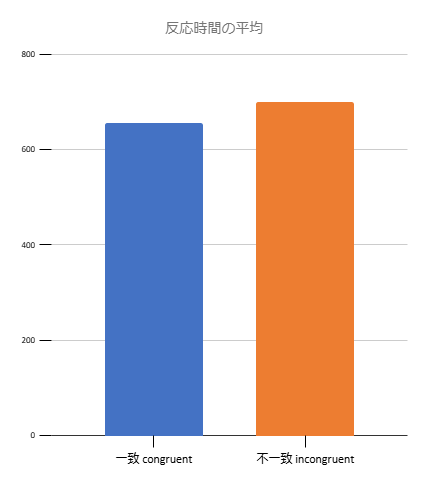
\includegraphics[keepaspectratio,width=6cm]{respons_speed.png}
%         \\[0cm]
%         \centering
%         \parbox{6cm}{\caption{反応時間の平均}}
%     \end{tabular}
% \end{wrapfigure}

\begin{figure}
    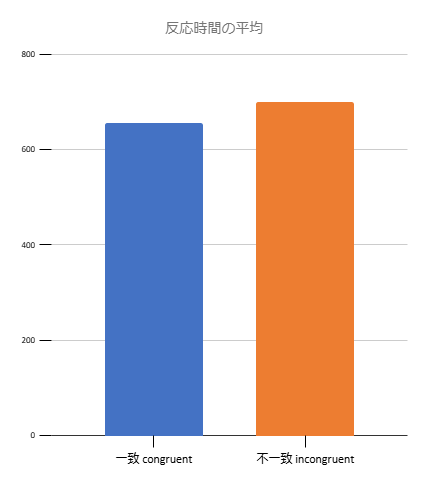
\includegraphics[width=7cm]{respons_speed.png}
    \centering
    \caption{反応時間の平均}
\end{figure}

集計したデータをから,色と意味が不一致の文字の色を答える場合の平均の反応時間がより長いことが分かる.
色と意味が一致の場合と不一致場合のデータに対して,対応有り,両側のt検定を適用したところ,p値は0.012であった.
これは有意水準0.05よりも小さい数値であり,一致と不一致には反応速度において有意な差が見られることが分かった.


\subsection{考察}

色と意味が一致している文字と不一致の文字の色を答える反応速度に有意な差が見られたことから,
一致と不一致には識別速度に有意な差があったと言っても良い.
そして,実際に有意な差が見られたことから,ストループ効果は効力があるということを強く支持する結果となった.

\subsection{結論}
色と意味の一致,不一致によって,識別速度に有意な差が見られ,不一致がより長い時間が必要であることが確かめられた.
これらの事実によって,色と意味が一致していない文字を目にしたとき,その文字の色を答えるのに時間がかかる可能性が高く,
ストループ効果が働いていると考えられる.


% =====================================================================================


\section{ウェブサイトのユーザビリティの評価とその分析}

\subsection{方法}

\subsubsection{評価データの取得}
ウェブサイトのユーザビリティの評価データを取得するために,4つのウェブサイトを用いてアンケート形式で実験を行った.
ウェブサイトには2つのカテゴリーがあり,同じカテゴリー同士のサイトAとサイトB,サイトCとサイトDを比較する形でデータを取得した.
アンケートにはGoogleフォームを使用した.また,各質問項目にリッカート尺度を用いることで参加者の定量的な評価を得られるようにしている.
質問項目は事前に準備された3つの質問と,講義中に割り振られた12個のグループが提案した12個の質問を合わせた計15個の項目がある.

\subsubsection{測定実験参加者}
サイト評価のアンケートには情報学群2年生が参加した.しかし,必ずしも全員のデータがあるとは限らない.

\subsubsection{分析に方法}
アンケート結果の処理において,有効なデータの抽出のためにPython及びそのライブラリ「Pandas」を使用した.また,
アンケート結果の分析にはR Studio,Excelを使用した.

サイトAB間の分析には質問項目15個の中から
\begin{enumerate}[label=\textbf{質問\arabic*.},leftmargin=2cm]
    \item 「このサイトには統一感があるか」
    \item 「このサイトの操作手順はシンプルでわかりやすいか」
    \item 「自分の条件に合った価格で表示させることができるか」
\end{enumerate}
の3つを使用した.

サイトCB間の分析には質問項目15個の中から
\begin{enumerate}[label=\textbf{質問\arabic*.},leftmargin=2cm]
    \item 「このサイトには統一感があるか」
    \item 「このサイトの操作手順はシンプルでわかりやすいか」
    \item 「求めている条件に合致する情報を見つけるまでの操作数が少ないか」
\end{enumerate}
の3つを使用した.

\subsection{結果}

\subsection{考察}

\subsection{結論}


% =====================================================================================


\section{カラーユニバーサルデザインに配慮したグラフデザインの考案}

\subsection{方法}
使⽤した機器・ソフトウェアの説明,⽬的を達成するために⾏なった具体的⼿続き,記録


\subsubsection{グループ単位での活動}
講義中に割り振られたグループごとにグラフデザインを考案した.

\subsubsection{使用するデータ}
商品の売り上げ等を模したデータをもとに事前に作成された円グラフと折れ線グラフが与えられた.
これらのグラフはカラーユニバーサルデザインが考慮されていないデザインで作成されている.

\subsubsection{作成方法}
グラフはJavaScriptとHTMLによって記述されており,ウェブブラウザにてグラフを描画することができる.
そして,グラフの作成は与えられたグラフを一部変更する形で行われた.
JavaScriptコードを適切に変更して,グループで一つのグラフデザインを作成する.

\subsubsection{デザインの評価}
作成したグラフがカラーユニバーサルデザインに配慮したデザインであるかを客観的に評価するために,
ImageJのVischeckPanelというプラグインを使用した.
VischeckPanelを用いることで1型,2型,3型の色覚異常の人間から観察されるグラフのデザインを描画することができる.
これを使用して,色覚型に寄らずに視覚情報からグラフの意味が容易に解釈できるか検証した.

\subsection{結果}
以下は作成した図について各色覚型での見え方を示している.

\begin{figure}[H]
    \begin{minipage}[b]{0.49\columnwidth}
        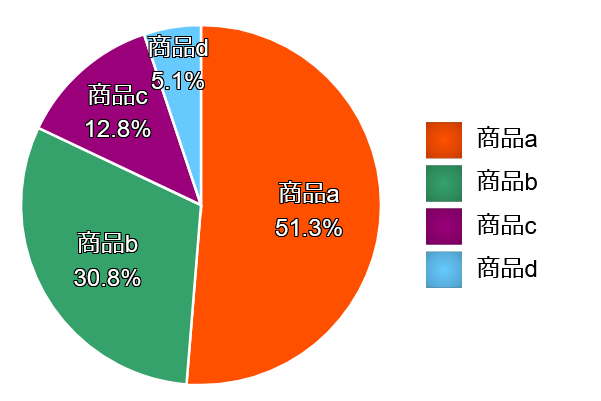
\includegraphics[width=6cm]{circle_fixed.png}
        \centering
        \caption{円グラフのC型色覚見え方}
    \end{minipage}
    \begin{minipage}[b]{0.49\columnwidth}
        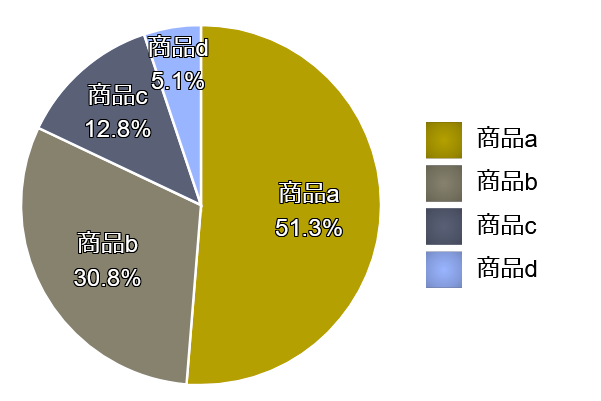
\includegraphics[width=6cm]{circle_fixed_deuteranope.png}
        \centering
        \caption{円グラフの1型色覚見え方}
    \end{minipage}
\end{figure}

\begin{figure}[H]
    \begin{minipage}[b]{0.49\columnwidth}
        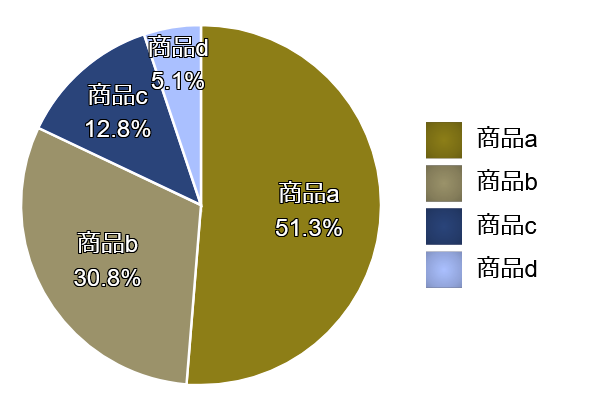
\includegraphics[width=6cm]{circle_fixed_protanope.png}
        \centering
        \caption{円グラフの2型色覚見え方}
    \end{minipage}
    \begin{minipage}[b]{0.49\columnwidth}
        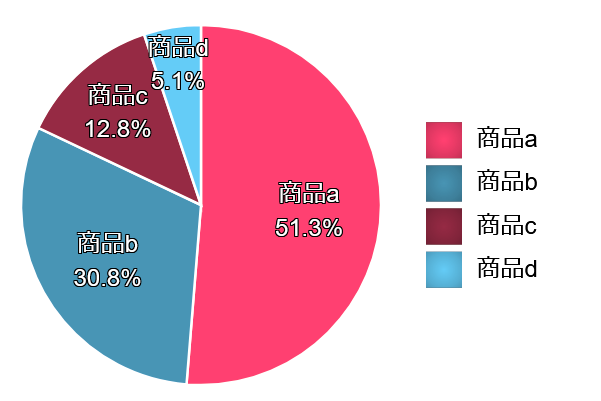
\includegraphics[width=6cm]{circle_fixed_tritanope.png}
        \centering
        \caption{円グラフの3型色覚見え方}
    \end{minipage}
\end{figure}

\begin{figure}[H]
    \begin{minipage}[b]{0.49\columnwidth}
        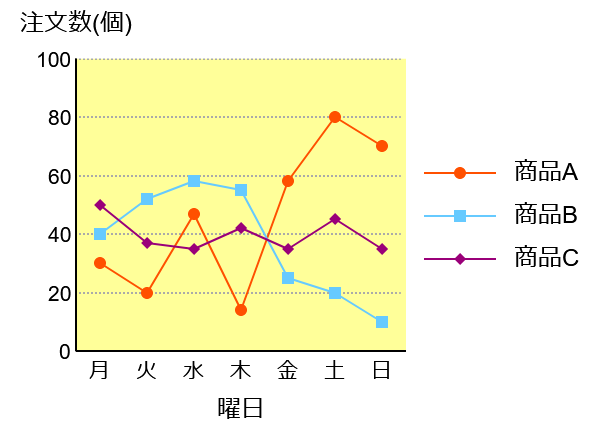
\includegraphics[width=6cm]{line_fixed.png}
        \centering
        \caption{折れ線グラフC型色覚見え方}
    \end{minipage}
    \begin{minipage}[b]{0.49\columnwidth}
        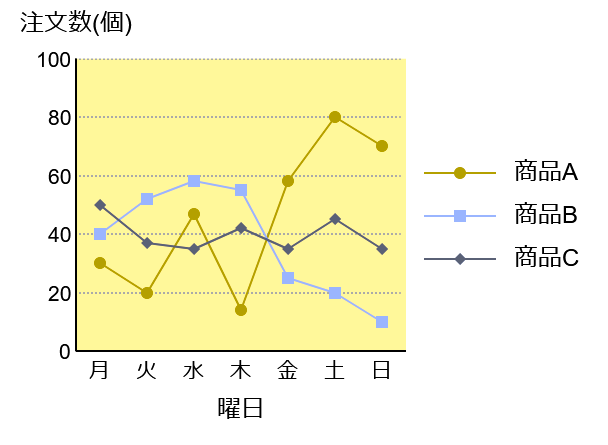
\includegraphics[width=6cm]{line_fixed_deuteranope.png}
        \centering
        \caption{折れ線グラフ1型色覚見え方}
    \end{minipage}
\end{figure}

\begin{figure}[H]
    \begin{minipage}[b]{0.49\columnwidth}
        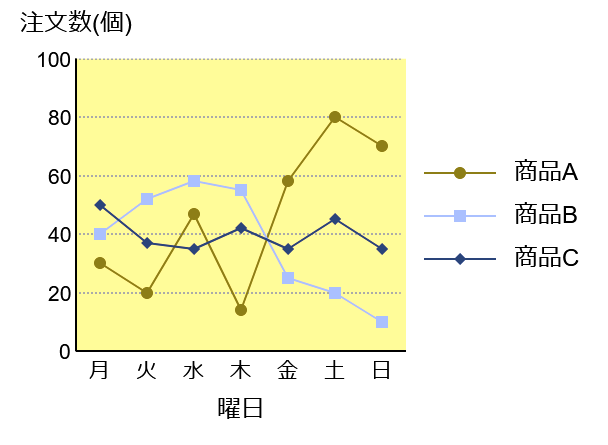
\includegraphics[width=6cm]{line_fixed_protanope.png}
        \centering
        \caption{折れ線グラフ2型色覚見え方}
    \end{minipage}
    \begin{minipage}[b]{0.49\columnwidth}
        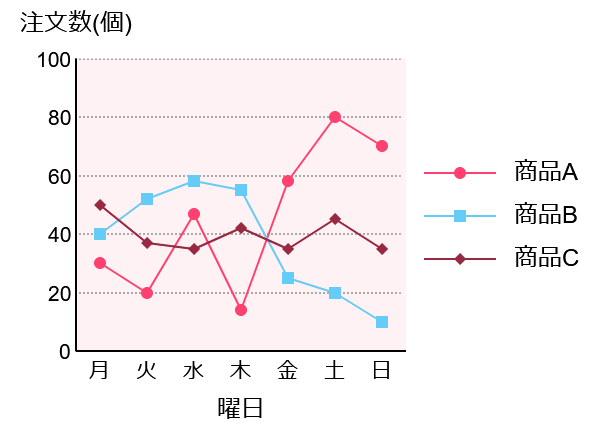
\includegraphics[width=6cm]{line_fixed_tritanope.png}
        \centering
        \caption{折れ線グラフ3型色覚見え方}
    \end{minipage}
\end{figure}

いづれの色覚型であっても色の判別がしやすい.
また,文字や記号も使用することで色だけに頼らずにグラフの情報を読み取れるように変更を加えた.


\subsection{考察}
\begin{figure}
    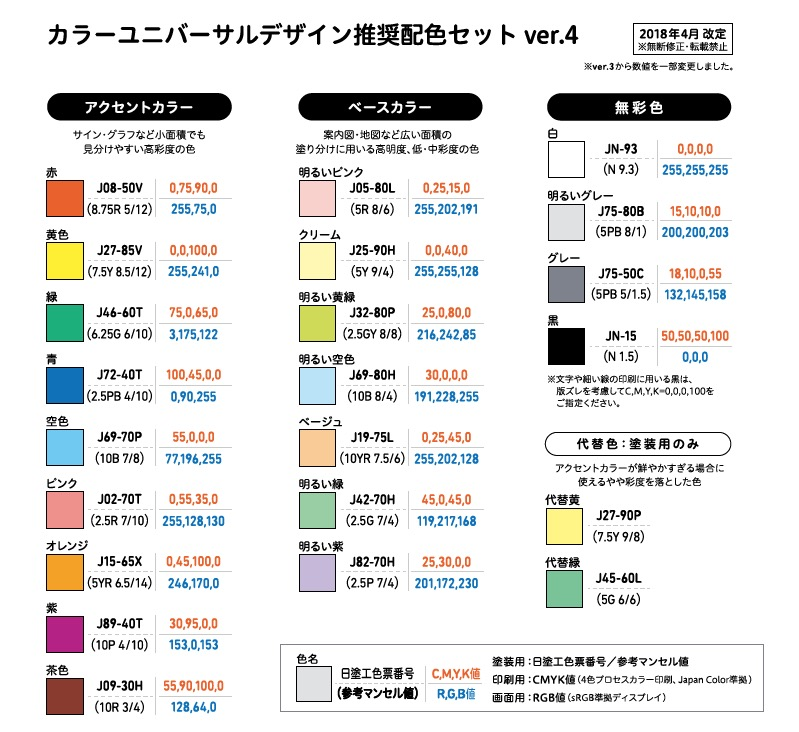
\includegraphics[width=8cm]{color_palet.jpg}
    \centering
    \caption{カラーユニバーサルデザインを配慮したカラーマップ}
\end{figure}

\subsection{結論}

\begin{thebibliography}{99}
    \bibitem{ms} Microsoftホームページ T.DIST関数 \url{https://support.microsoft.com/ja-jp/office/t-dist-%E9%96%A2%E6%95%B0-4329459f-ae91-48c2-bba8-1ead1c6c21b2}
    \bibitem{color_palet} NPO法人カラーユニバーサルデザイン機構 \url{https://cudo.jp/?page_id=1565}
\end{thebibliography}

\end{document}